\chapter{Network Function Virtualization}

\[
  NFV \neq SDN 
\]
Even though the definitions were similar a few years ago, they are not the same thing. NFV is about virtualizing network functions, while SDN is about virtualizing the network itself; however, they work nicely together.

\section{Introduction and context}
In typical enterprise networks, there aren't only servers and switches, but also a lot of network functions, such as firewalls, load balancers, intrusion detection systems, etc. These functions are usually implemented in dedicated hardware, which is expensive and hard to manage; besides these components have a strict chaining/ordering, that must be reflected in the network topology.\\
\ul{NFV is about moving these functions to software, so they can be run on commodity hardware.
}

NFV is one (the?) way to address these challenges by leveraging virtualization technologies. 
The main idea is \textbf{decoupling} physical network equipment from the functions that run on them, with network functions provided as \textbf{plain software}.

A Network service can be decomposed into a set of \textbf{Virtual Network Functions} (\texttt{VNF}s).
VNFs may then be relocated and instantiated at different network locations without requiring to buy and install new hardware.

One of the key points is to \textbf{reduce costs}. Two types of costs are involved:
\begin{itemize}
   \item \textbf{CAPEX} (Capital Expenditure): the cost of buying the hardware.
   This is reduced by buying general purpose hardware instead of specialized one.
   \item \textbf{OPEX} (Operational Expenditure): the cost of managing the hardware.
   Reduced by reducing the number of devices to manage.
\end{itemize}

Performance is also a concern, as the software implementation may be slower than the hardware one. However, the performance of commodity hardware is increasing, and the software can be optimized to run on it.

\framedt{Benefits}{
   \begin{itemize}
      \item Improved resource usage efficiency
      \begin{itemize}
         \item Due to flexible allocation of different NFs on the HW pool
      \end{itemize}
      \item Elasticity
      \begin{itemize}
      \item Capacity dedicated to each NF can be dynamically modified (scaling)
         according to actual load on the network
      \end{itemize}
      \item Topology reconfiguration
      \begin{itemize}
         \item Network topology can be dynamically reconfigured to optimize
         performance
      \end{itemize}
   \end{itemize}
   \begin{center}
      \begin{tikzpicture}
         \draw[-implies,double equal sign distance] (0,0) -- (0,-0.8);
      \end{tikzpicture}\\
      \textit{Higher service availability and resiliency}\\
   \end{center}
}

\section{Network Service}
An end-to-end network service can be defined as a forwarding graph of network
functions and end points/terminals;
So it can be viewed architecturally as a forwarding graph of Network Functions (NFs) interconnected by the supporting network infrastructure.
Nodes running VNFs are called \textbf{Points of Presence} (\textit{PoPs}) and are interconnected by logical links, backed by the underlying the network infrastructure physical links.

\begin{figure}[htbp]
   \centering
   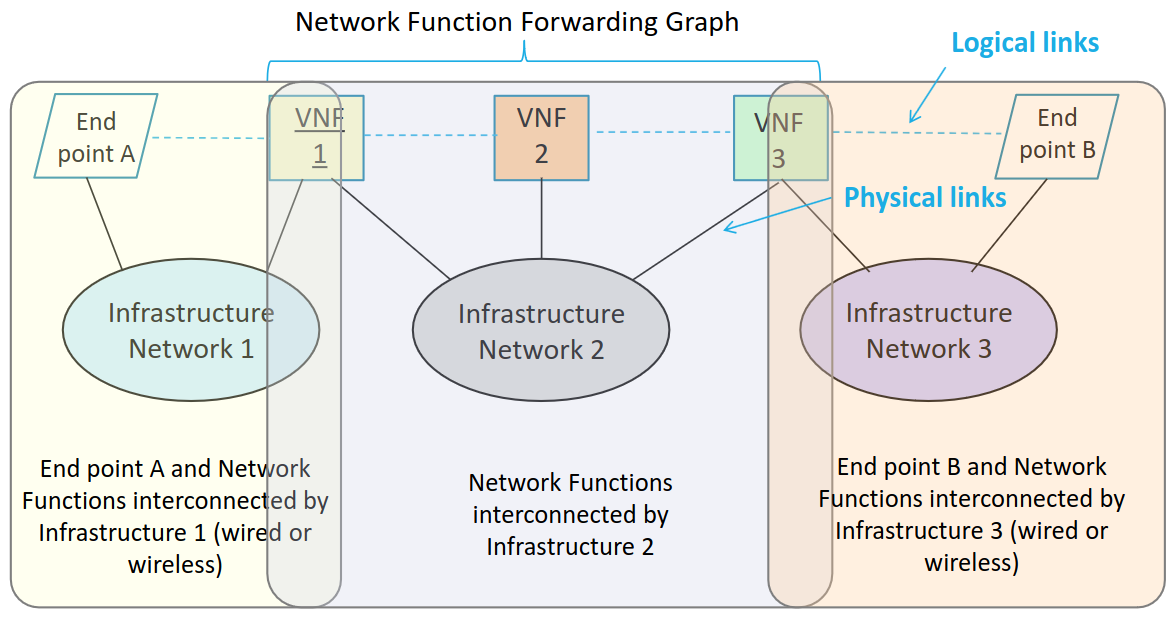
\includegraphics{images/VNF_service_infr.png}
   \caption{VNF Network Service}
   \label{fig:VNF_service}
\end{figure}

\begin{figure}[htbp]
   \centering
   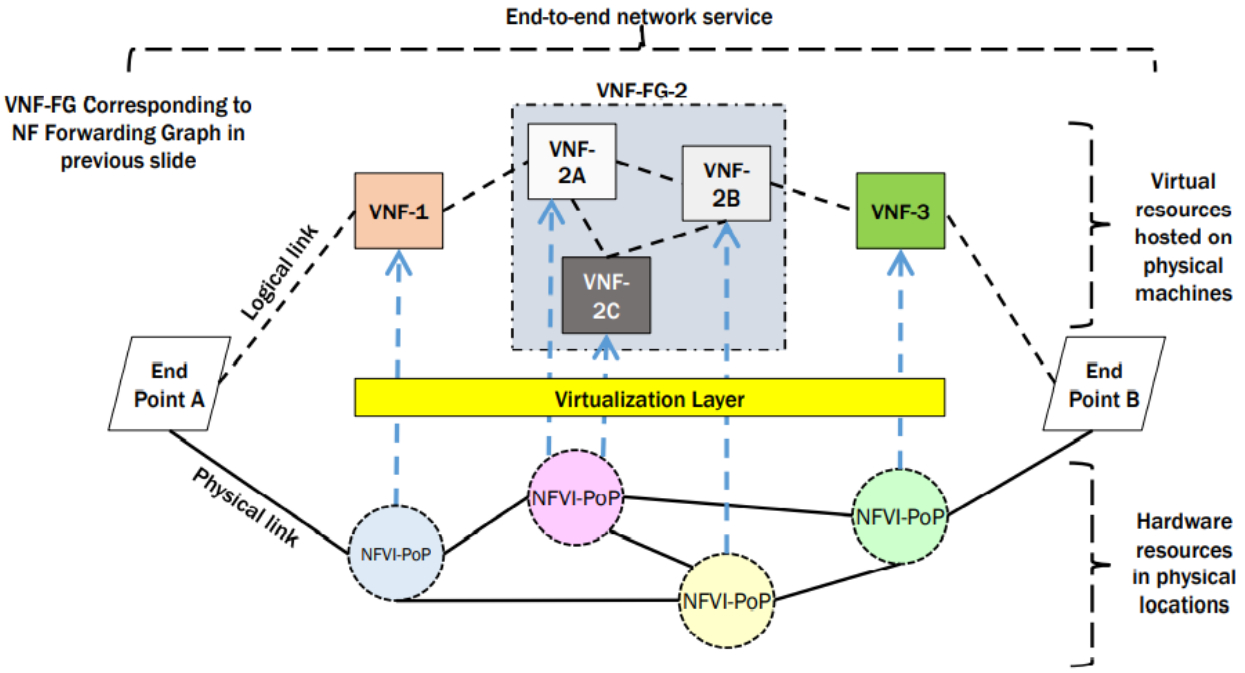
\includegraphics{images/vnf_fullarch.png}
   \caption{VNF more complete example}
   As displayed in figure a single PoP may run multiple VNFs.
   Logical links between VNFs may be managed using SDN, and must be backed by physical links in the underlying network infrastructure.
   \label{fig:vnf_fullarch}
\end{figure}

\section{NFV Architectural Framework}

\colfill
\begin{paracol}{2}
   \begin{figure}[htbp]
      \centering
   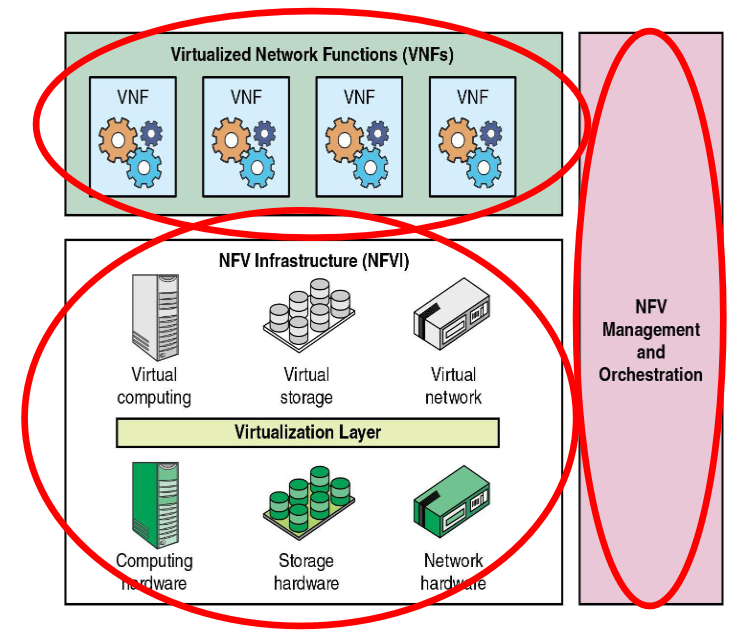
\includegraphics{images/NFV_architecture.png}
   \caption{NFV Architecture}
   \label{fig:NFV_architecture}
\end{figure}
\colfill

\switchcolumn
\colfill
\begin{itemize}
   \item \textbf{NFV} infrastructure (NFVI)\\
   Comprises the hardware and software resources that create the environment in which VNFs are deployed.
   \item \textbf{VNF}\\ 
   The collection of VNF implemented in software to run on virtual computing, storage, and networking resources.
   \item \textbf{NFV management} and \textbf{Orchestration} (NFV-MANO)\\
   Framework for the management and orchestration of all resources in the NFV environment.
\end{itemize}
\colfill
\end{paracol}

\begin{paracol}{2}
   \colfill
   \begin{figure}[htbp]
      \centering
      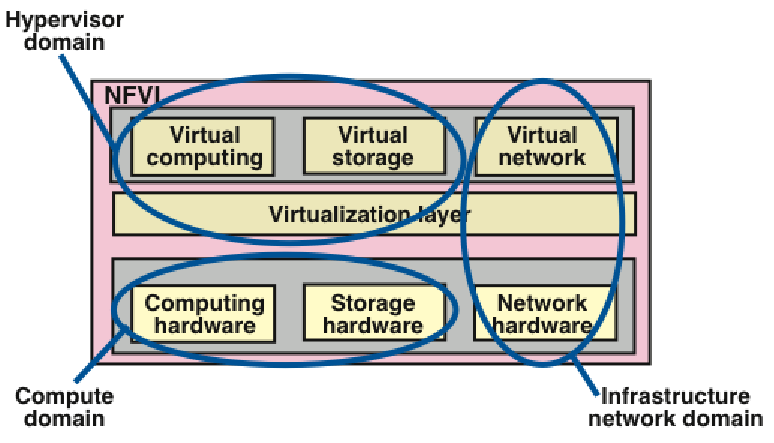
\includegraphics{images/NFV_infr.png}
      \caption{NFV Infrastructure}
      \label{fig:NFV_infr}
   \end{figure}
   \colfill
   \switchcolumn
   \colfill
   The NFV infrastructure is the typical hardware plus virtual machines managed by a hypervisor.
   The three domains depicted in Fig. \ref{fig:NFV_infr} are:
   \begin{itemize}
      \item \textbf{Compute Domain}\\
      Provides commercial off-the- shelf (COTS) high-volume servers and storage.
      \item \textbf{Hypervisor Domain}\\
      Mediates the resources of the compute domain to the VMs (today also Containers) of the software appliances, providing an abstraction of the hardware.
      \item \textbf{Infrastructure Network Domain}\\
      Comprises all the generic high volume switches interconnected into a network that can be configured to supply network services
   \end{itemize}
   \colfill
\end{paracol}

\subsection{vSwitch - Case study}
\textbf{Virtual Switches} provide connectivity between \textit{Virtual Interfaces} (VIFs) and the \textit{Physical Interfaces} (PIFs), and also handle traffic between VIFs located on the same host.\\
A virtual switch is a software program that emulates a switch (Layer 2 device).

\subsection{VNF Placement problem}
Placing a chain of VNFs is hard, and consists of maximing a utility function, while respecting infrastructure constraints and QoS requirements. The utility function is usually a combination of:
\begin{itemize}
   \item Minimization of the overall delay;
   \item Minimization of deployments costs,
   \item Maximization of remaining bandwidth, etc.
\end{itemize}

\section{NFV MANO}

\begin{figure}[htbp]
   \centering
   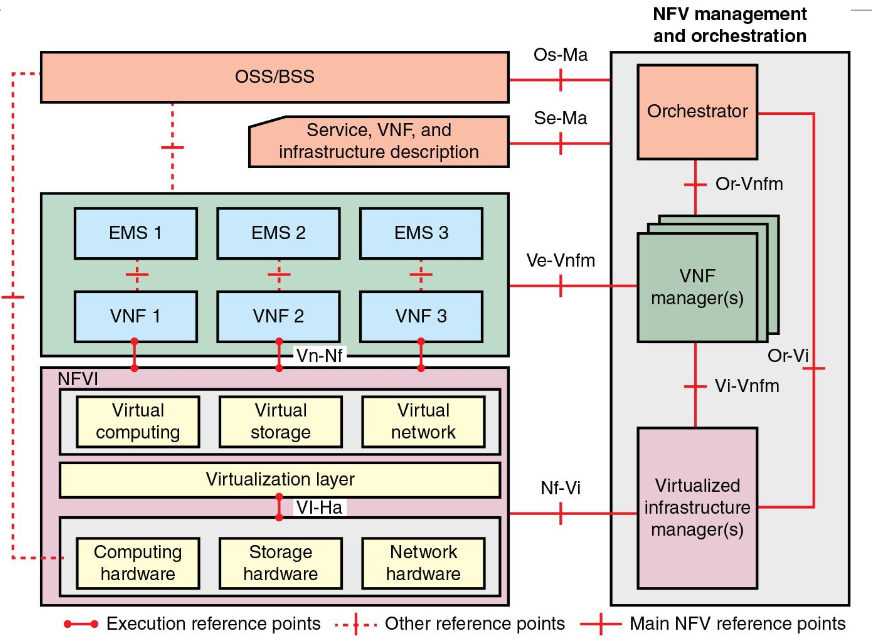
\includegraphics{images/NFV_mano.png}
   \caption{NFV Reference - Architectural Framework}
   Here VNF1,2,3 are VNF instances, EMS1,2,3 are Element Management Systems, and OSS/BSS is the traditional network management,
   \label{fig:NFV_mano}
\end{figure}

\begin{itemize}
   \item Oversees the provisioning of the VNFs,
   and related operations
   \begin{itemize}
      \item The configuration of the VNFs, and
      \item The configuration of the infrastructure the VNFs run on
   \end{itemize}
   \item Includes orchestration and lifetime management of physical and/or software resources supporting the infrastructure virtualization and the lifecycle management of VNFs
   \item Includes databases used to store information and data models defining deployment and lifecycle properties of functions, services and resources
   \item Defines interfaces used for communications between components of the MANO, as well as coordination with traditional network management, such as OSS/BS
\end{itemize}

\subsection*{VIM - Virtualized Infrastructure
Management}
VIM comprises the functions that are used to control and manage the interaction of a VNF with computing, storage, and network resources under its authority, as well as their virtualization.

A VIM is responsible for controlling and managing the NFVI compute, storage, and network resources. 
\note{A ---whole--- MANO may orchestrate multiple VIMs.}

\subsection*{Virtual Network Function
Manager - VNFM}
Oversees lifecycle management (e.g. instantiation, update, query, scaling, termination) of VNF instances.

\subsection*{NFV Orchestrator - NFVO}
Responsible for installing and configuring new network services (NS) and virtual network function (VNF) packages, NS lifecycle management and global resource management.\\
Acts also as network service orchestrator, managing/coordinating the creation of an end-to-end service that involves VNFs.